\documentclass[12pt,a4paper]{article}
\usepackage{fullpage}
\usepackage[margin=2cm]{geometry}
\usepackage{amsmath}
\usepackage{subfig}
\usepackage{graphicx}
\usepackage[justification=centering]{caption}
\begin{document}
\title{A comparison of two convolutional neural networks for landmarks detection }
\author{LE Van Linh and BEURTON-AIMAR Marie}
\date{October, 2017}
\maketitle
\begin{abstract}
	In this study, we presented a comparison between two convolution neural networks (CNNs) which are used to predict the landmarks on biological images. The first model was presented by Celia Cintas et al\cite{cintas2016automatic}. The model is used to predict the 45 landmarks on the human ear. The second model is proposed by us as a result of tutorial about Lassagne framework\cite{lasagne}. The proposed model is designed to predict 8 landmarks on beetle's pronotum. Both models have experimented on the dataset of pronotum images and have implemented by Python on Lassagne framework. Besides, we also present another way to augment the data for CNN.
\end{abstract}
\section{The models}
In this section, we will describe the architecture of the models and the parameters that used during training and validation processes.
\subsection{Model 1: Automatic ear landmarks detection}
\subsubsection{Architecture}
Celia Cintas et al\cite{cintas2016automatic} proposed a method based on geometric morphometric and deep learning for automatic ear detection and feature extraction in the form of landmarks. The convolutional neural network was trained with a set of manually landmarks examples. The network is able to provide the morphometric landmarks on ear image automatically.

Three models were designed and trained for performing the automatic landmarks task. These architectures are different in the number of convolution layers, the filter sizes, and the learning rate. The data which used by the network for training and validation is a set of gray-scale images of the size $96 \times 96$ and set of list of manual landmarks coresponding to all the images in the image dataset.% Before giving to the network, the brightness of the image is scaled to $[0,1]$, instead of $[0,255]$ and the landmark coordinates is normalized to $[-1,1]$, instead of $[0,96]$.

\textbf{Fig.\ref{1Econv}} shows the best architecture of three models. In this architecture, a structure of two convolutional layers with the filters, followed by maximum pooling and dropout layer. This structure is repeated \textbf{three times} to obtain features at different levels with different size of filters(i.e $4 \times 4$ and $3 \times 3$). After extraction the features, two fully connected linear layers with 1500 units each and a dropout layer is hired. The output layer contains 90 output units corresponding with 45 landmarks for the predicted position of the landmarks. But in our case, the output of the last layer has changed from $90$ to $16$ for adapting with the number of landmarks on pronotum.
\begin{figure}[h!]
	\centering
	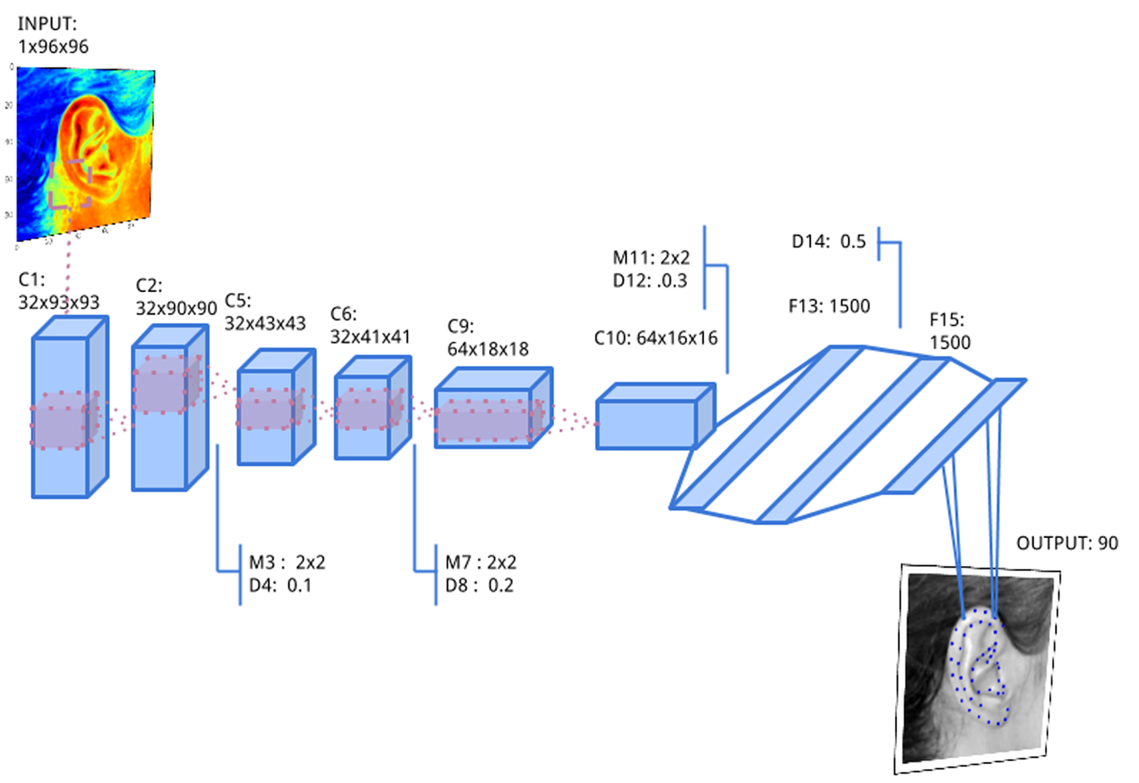
\includegraphics[scale=0.4]{images/ear_cnn}
	\caption{The best architecture for automatic ear's landmarks detection}
	\label{1Econv}
\end{figure}
\subsubsection{Parameters}
The network was trained with $5000$ \texttt{epochs} and \texttt{batch size} of $128$. For each epoch, the dataset is randomly split into the training set and validation set. The number of images in the sets is divided with the ratio of $80\%:20\%$, respectively. The \texttt{learning rate} is set to $0.03$; and the initial of \texttt{momentum} is $0.9$. During training, the learning rate and momentum are re-calculated to adjust with the number of remaining epochs. All the parameters in model 1 are shown in Table.\ref{celiaparameters}:
\begin{table}[h!]
	\centering
	\begin{tabular}{l l l}
	Parameter & Initial value & End value \\ \hline
	Epochs & 5000 &  \\ \hline
	Training batch size & 128 & \\ \hline
	Testing batch size & 128 & \\ \hline
	Learning rate & 0.03 & 0.00001 \\ \hline
	Momentum & 0.9 & 0.9999 \\ \hline
	\end{tabular}
	\caption{The network parameters in the Celia model}
	\label{celiaparameters}
\end{table}~\\
\subsection{Model 2: Automatic beetle landmarks detection}
\subsubsection{Architecture}
From the tutorial of Daniel Nouri\footnote{http://danielnouri.org/} about using CNN to detect facial key points. We propose a CNN to detect the landmarks on pronotum. The proposed network includes three convolutional layers followed by three maximum pooling layers and three full connected layers(Fig.\ref{pmodel}). The network receives the gray-scale image ($256 \times 192$) as the input. The deep of convolutional layers is increased from $32, 64, $ to $ 128$ with different size of filter. The size of filters in pooling layers are kept in the same size of $2 \times 2$. At the end of network, three full-connected layers with the size of $500, 500, $ and $16$ are set up to predict the positions of landmarks. Besides, the model is designed with a small sharing learning-rate and the momentum. The learning-rate and the momentum are changed overtime of training.
\begin{figure}[h!]
	\centering
	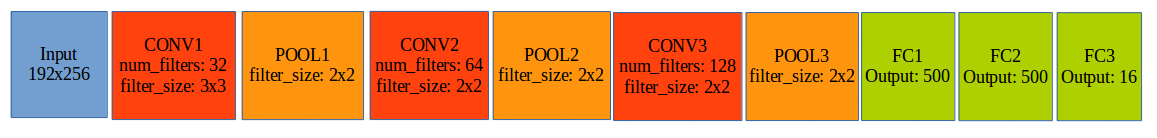
\includegraphics[scale=0.4]{images/model3}
	\caption{The architecture of proposed model}
	\label{pmodel}
\end{figure}
\subsubsection{Parameters}
The parameters in model 2 are shown in the Table.\ref{model2parameters}:
\begin{table}[h!]
	\centering
	\begin{tabular}{l l l}
	Parameter & Initial value & End value \\ \hline
	Epochs & 5000 &  \\ \hline
	Training batch size & 128 & \\ \hline
	Testing batch size & 128 & \\ \hline
	Learning rate & 0.03 & 0.0001 \\ \hline
	Momentum & 0.9 & 0.9999 \\ \hline
	\end{tabular}
	\caption{The network parameters in proposed model}
	\label{model2parameters}
\end{table}~\\
\section{Data}
\label{sectionData}
The experiment data includes 293 color images of pronotum. The images are divided into 3 subsets: training($200$ images), validation($60$ images) and testing set($33 images$). In which, the training and validation are combined to use as the input data of the networks(total $260$ images). The images in testing set are used to evaluate the model. The images are chosen randomly to put into each set (after we have done some experiments).

Because the number of the images are limited (just $260$ color images), it does not enough to use for training process. Additional, the models are worked on gray-scale images. So, we applied some rules to enlarge the dataset. The first rule is adding a constant value to a channel of RGB image, we will have a new RGB image. For example, from an original $RGB$ image, if we add $10$ to red channel, we will have a new image $(R+10)GB$. Then, we apply the same rule with blue and green channel, we will obtain two new images: $R(G+10)B$ and $RG(B+10)$. By that way, from an RGB image, we can generate three RGB images by adding a constant to each channel(each time just change to a channel). The second rule is splitting the channels of RGB image (because the models work on gray-scale). It means that we can generate six versions from an original image. At the end, the number of the image in the training data is $ 260 \times 7 = 1820$ images (six versions and original). Before giving to the models, the images are down-sampled with the size of $256 \times 192$. The number of the images in training set and validation set are splitted automatically by the model's parameter.
\section{Experiments}
In this section, we describe the experiment processes of two models on pronotum dataset (section \ref{sectionData}). The experiments were conducted in the way pre-processing data before giving to the network. Then, some improvements are added into model 3 to obtain the better result.
\subsection{Experiment 1}
\subsection{Experiment 2}
\subsection{The improvements on model 3}

\section{Model 1 and model 2 on pronotum}
\subsection{Dataset preparing}
The dataset includes 293 pronotum images. The images are divided into three subsets: the training set (200 images), the validation set (60 images) and the testing set (33 images). Because the dataset is limited and the models are worked on gray-scale images, we applied some ways to en-large the dataset. Firstly, for each original image in RGB, each channel is modified by adding some values. Secondly, the channels of the original image are split. So, we have obtained 1400 images for the training set and 420 images for the validation set. At the end, the images are down-sampled with the  size of $256 \times 192$ before giving to the networks.

%To enlarge the dataset during training, the image in training and validation set are augmentation by modifying the valued of red and green channel. So, at the end, we have 600 and 180 images in training and validation set, respectively.
\subsection{Model 1 and pronotum landmarks}
The networks in the first level are modified to suitable with the prediction of landmarks on the pronotum (8-landmarks). For each pronotum, eight manual landmarks have been set. The bounding box is created depending on the coordinate of the manual landmark and kept with the same size. The networks in the first level are used as followed:
\begin{itemize}
	\item F1 network recognizes whole pronotum bounding box with eight landmarks.
	\item EN1 network predicts the location of the first five-landmarks i.e $[1..5]$.
	\item NM1 network is used to estimated the position of last four-landmarks and the first landmark i.e $[5..8,1]$.
	\item At the end, the position of each landmark is average of the predicted position in the networks.
\end{itemize} 
\subsubsection{Testing}
During training, the Euclidean distance (sum of squares) is used to compute the loss of the networks. The error rate of each network during training is shown in the Table.\ref{model1p}:\\
\begin{table}[h!]
	\centering
	\begin{tabular}{l r}
	Network & Loss \\ \hline
	F1 & 0.013 \\ \hline
	EN1 & 0.47\\ \hline
	NM1 &  0.5
	\end{tabular}
	\caption{The loss of the networks in Model 1 on pronotum dataset}
	\label{model1p}
\end{table}
\begin{figure}[h!]
\centering
\subfloat[Test 1]{\label{}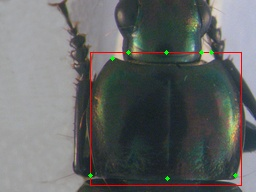
\includegraphics[width=0.2\textwidth]{./images/test1}}~~
\subfloat[Test 2]{\label{}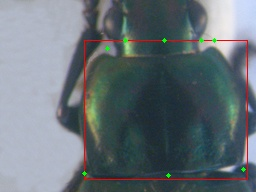
\includegraphics[width=0.2\textwidth]{./images/test2}}\\
\subfloat[Test 3]{\label{}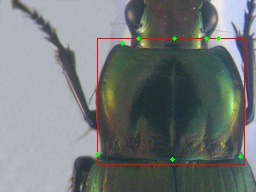
\includegraphics[width=0.2\textwidth]{./images/test3}}~~
\subfloat[Test 4]{\label{}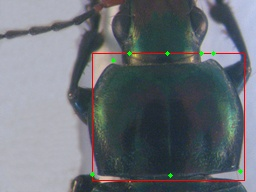
\includegraphics[width=0.2\textwidth]{./images/test4}}\\
\caption{The pronotum with predicted landmarks at level 1}
\label{model1pTest}
\end{figure}\\
From Table \ref{model1p}, the errors of EN1 and NM1 are still high. That errors make the prediction result of level 1 do not enough good. Besides, the networks at level 2 and level 3 used the prediction at level 1 as the input data to predict the new position. So, we can not continue with the level 2, 3 until the result at level 1 is improved. Perhaps, the model in model 1 is not suitable to detect the landmarks on pronotum.  Fig. \ref{model1pTest} shows the prediction landmarks on four images. Followed that, the networks can detect the landmarks at positions 4, 5 and 7; the different positions still not good.
\subsection{Model 2 and pronotum landmarks}
The dataset is kept the same with model 1 (1400 images for training and 420 images for validation) but having some changes. Firstly, the ways to choose the data(to train and validate) is changed. All images are combined. Then, the network will automatically choose $75 \%$ data to train and $25 \%$ for validation. Secondly, the inputs that given to the network are just the image and landmarks(without the coordinates of the bounding box).

The network is run 3000 iterations with the learning rate begin from $0.08$ to $0.01$. During training, the learning rate is changed to fit with the remaining iterations\cite{lecun2012efficient}. Fig.\ref{model2pl} shows the first 700 iterations during training. The loss did not have many changes after $100^{th}$ iteration.

\begin{figure}[h!]
	\centering
	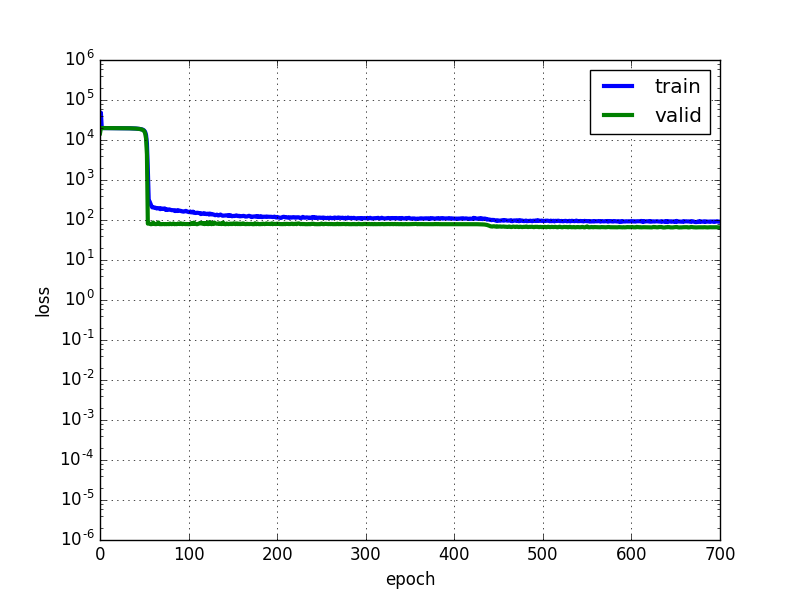
\includegraphics[scale=0.4]{images/figure_1_loss_celia}
	\caption{The losses of model 2 on pronotum dataset}
	\label{model2pl}
\end{figure}

\begin{figure}[h!]
	\centering
	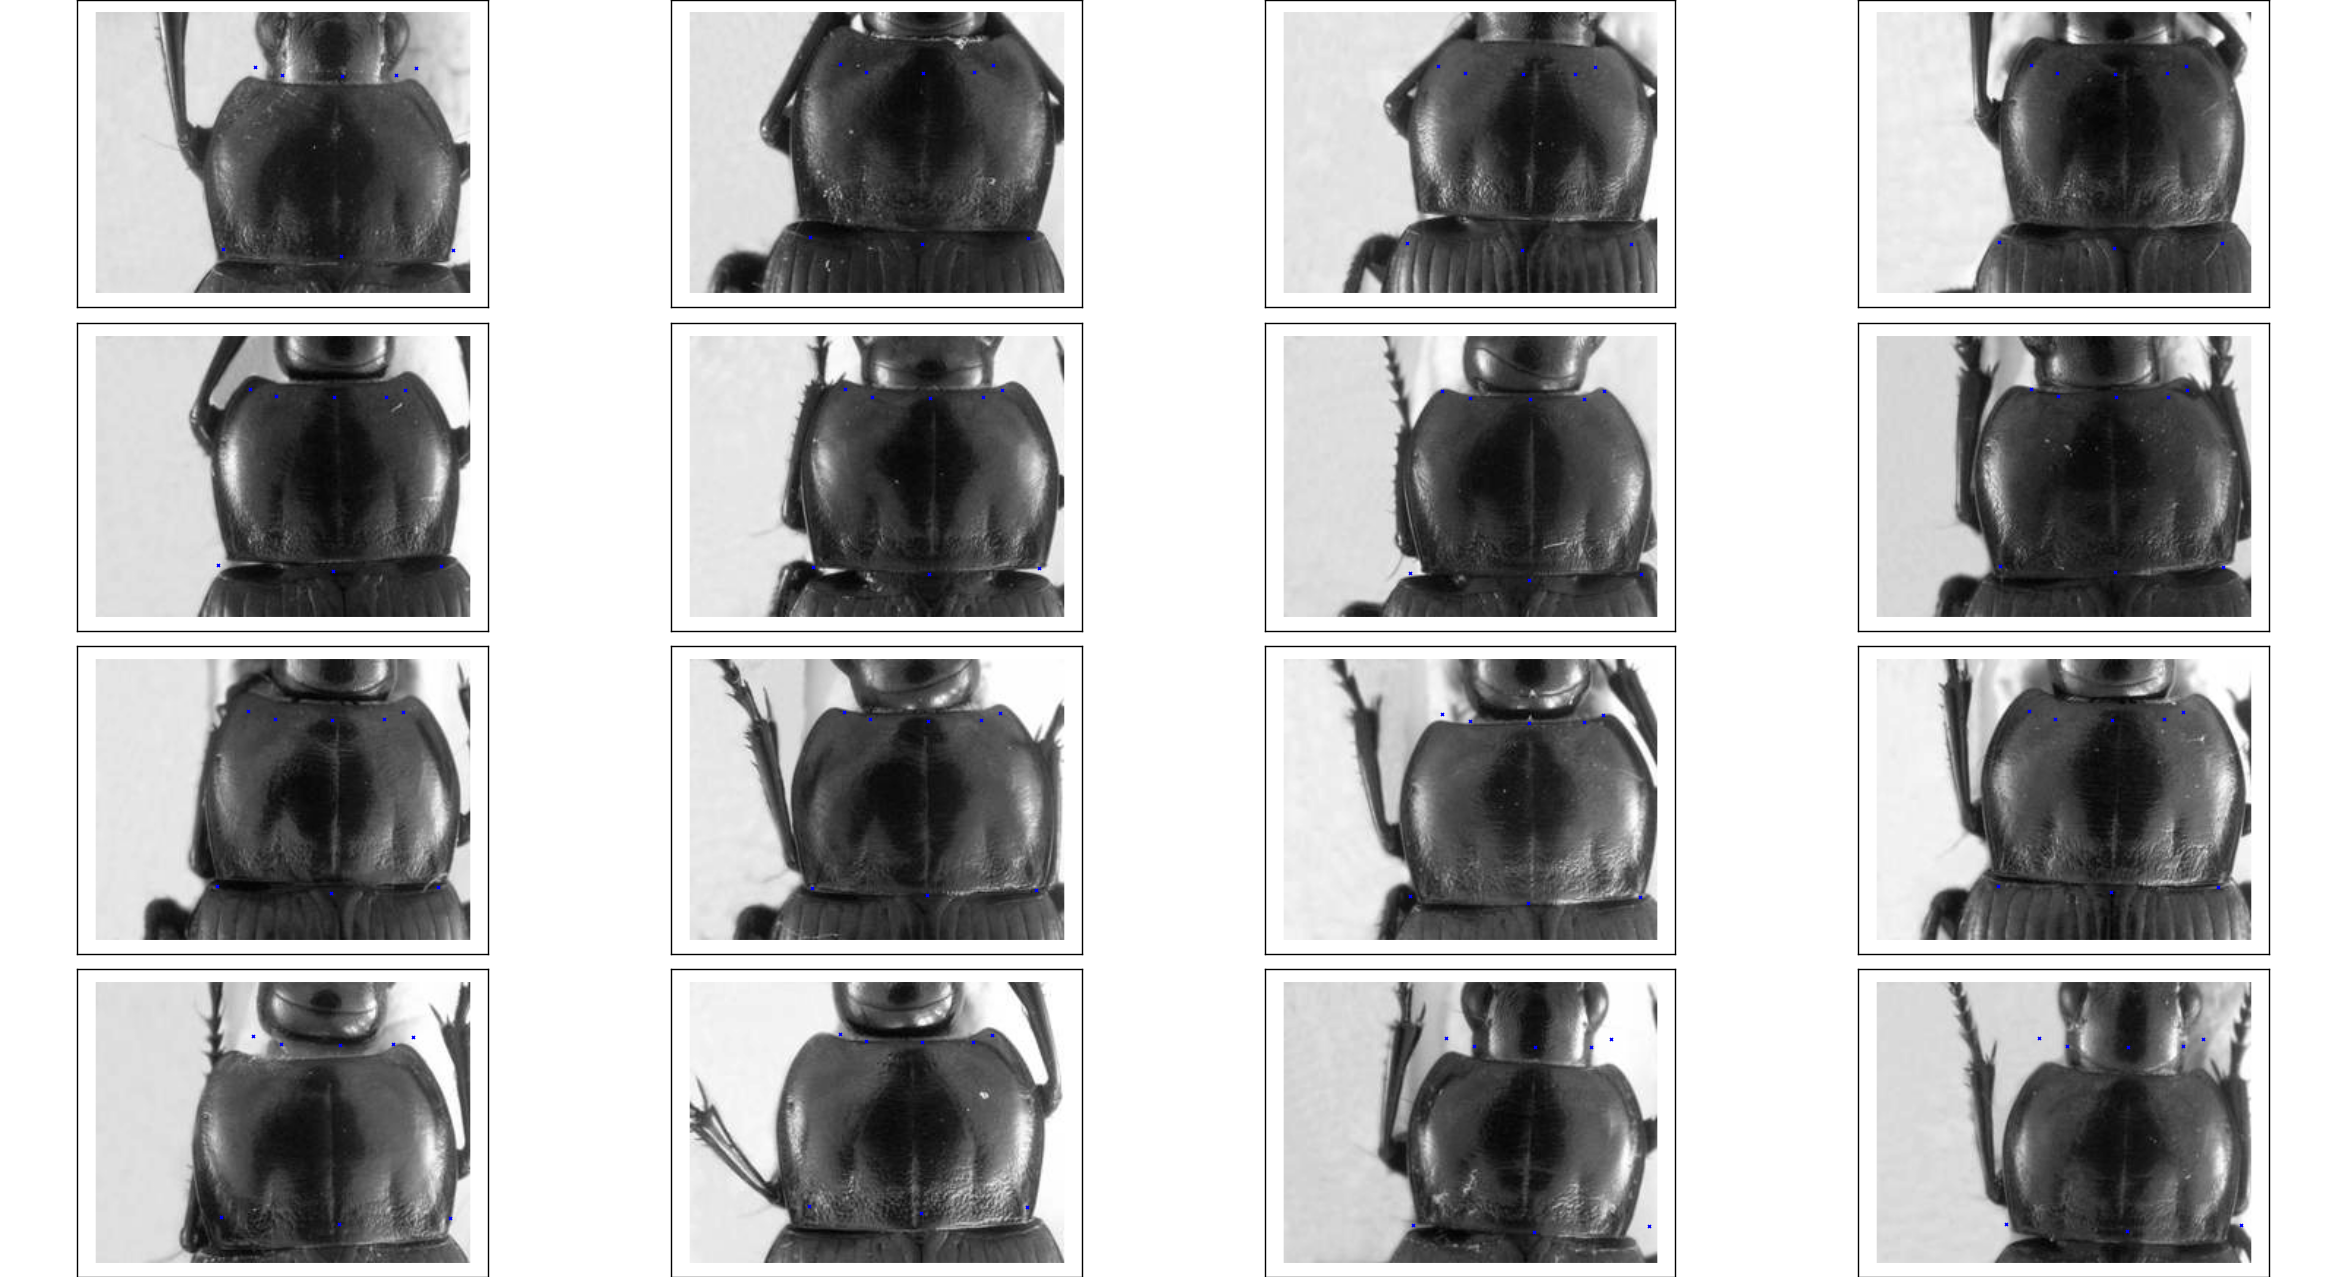
\includegraphics[scale=0.25]{images/figure_1_celia}
	\caption{The prediction landmarks on pronotum of model 2}
	\label{model2pt}
\end{figure}
Fig.\ref{model2pt} shows the prediction landmarks on 16 images. Following, the prediction landmarks from the network of model 2 are closed with the pronotum but the location is still inaccurate.

%\subsection{Comparing model 1 and model 2}
%Table C shows some differences from 2 models
%\begin{table}[h!]
%	\centering
%	\begin{tabular}{l c c c}
%	Model & Framework & Dataset (images) & Learning rate \\ \hline
%	Model 1 & Caffe & 13466 & 0.013 \\ \hline
%	Model 2 & Lasagne(Theano) & 2140 & zz\\
%	\end{tabular}
%\end{table}\\
\section{Proposed architecture (model 3)}
\subsection{Model and parameters}
From the tutorial of Daniel Nouri\footnote{http://danielnouri.org/} about using CNN to detect facial key points. We propose a CNN to detect the landmarks on pronotum. The proposed network includes three convolutional layers followed by three maximum pooling layers and three full connected layers(Fig.\ref{pmodel}). The network receives the gray-scale image ($256 \times 192$) as the input. The deep of convolutional layers is increased from $32, 64, $ to $ 128$ with different size of filter. The size of filters in pooling layers are kept in the same size of $2 \times 2$. At the end of network, three full-connected layers with the size of $500, 500, $ and $16$ are set up to predict the positions of landmarks. Besides, the model is designed with a small sharing learning-rate and the momentum. The learning-rate and the momentum are changed overtime of training.
\begin{figure}[h!]
	\centering
	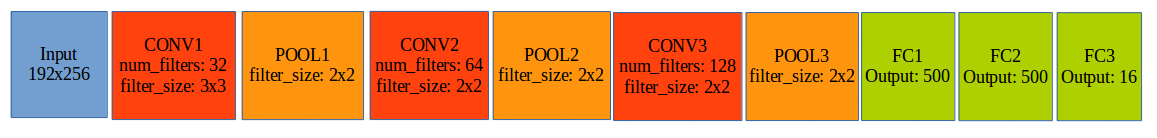
\includegraphics[scale=0.4]{images/model3}
	\caption{The architecture of proposed model}
	\label{pmodel}
\end{figure}
\subsection{Training and experiments}
The model is trained with 1820 images in 5000 iterations. The images are normalized before giving to the network by scaling the intensity value to [0,1], instead of 0 to 255. The target values (x and y coordinates) is kept as original. During the training, the root-mean-square error (MSE) is used to calculate the loss.

To evaluate the stability and confidence of the model, we proposed several rules to select the images for the network, as Table.\ref{choosedata}:\\
\begin{table}[h!]
	\centering
	\begin{tabular}{c l l}
	Rule & Test set & Training and validation set \\ \hline
	rule\_1 & From $1^{st}$ image to $33^{rd}$ image & Remaining images \\ \hline
	rule\_2 & From $260^{th}$ image to $293^{rd}$ image & Remaining images\\ \hline
	rule\_3 & Random & Random \\ \hline
	rule\_4 & From $90^{th}$ image to $122^{nd}$ image & Remaining images\\ \hline
	rule\_5 & From $200^{th}$ image to $232^{nd}$ image & Remaining images \\ \hline
	\end{tabular}
	\caption{The rules to choose the data for the network}
	\label{choosedata}
\end{table}~\\
Following the rules to choose the data, the loss of training and validation is shown in Table \ref{losschoosedata}. From the results in the table, the training losses in the cases of \textit{rule\_4, rule\_5} are smaller than other rules; but the validation losses are stability. It means the overfitting is appeared clearly in the case of \textit{rule\_4} and \textit{rule\_5}. In which, the smallest difference value between training and validation loss is belong to \textbf{random} case.
\begin{table}[h!]
	\centering
	\begin{tabular}{c l l}
	Rule & Training loss & Validation loss \\ \hline
	rule\_1 & $0.12739$ & $0.63681$ \\ \hline
	rule\_2 & $0.15204$ & $0.59480$ \\ \hline
	rule\_3 & $0.16694$ & $0.55584$ \\ \hline
	rule\_4 & $0.08798$ & $0.61934$ \\ \hline
	rule\_5 & $0.0918$ & $0.52843$ \\ \hline
	\end{tabular}
	\caption{The training loss and validation loss following each rule to choose the data}
	\label{losschoosedata}
\end{table}~\\[0.1cm]
Fig.\ref{cnn3l} shows the training curve loss and validation curve loss of the model on each rule to choose the data. From the beginning, the loss is not changed. When the training is longer and the learning rate is improved, the loss is decreased and a large distance between training and validation is appeared (over-fitting) but it is not that bad.

The model is tested on the test datasets(five rules). Then, correlation between the manual landmarks and predicted landmarks is computed by applying the correlation methods (see Table.\ref{pearson}, \ref{spearman}, \ref{kendall})
\begin{table}[h!]
	\centering
	\begin{tabular}{c c c}
		Rule & x correlation & y correlation \\ \hline
		rule\_1 & $0.9953877$ & $0.9941767$ \\ \hline
		rule\_2 & $0.9968787$ & $0.9960827$ \\ \hline
		rule\_3 & $0.9966784$ & $0.9957729$ \\ \hline
		rule\_4 & $0.9975662$ & $0.9985097$ \\ \hline
		rule\_5 & $0.9972048$ & $0.9976416$ \\ \hline
	\end{tabular}
	\caption{The correlation between manual and predicted landmarks by Pearson\cite{pallant2013spss} method}
	\label{pearson}
\end{table}
\begin{table}[h!]
	\centering
	\begin{tabular}{c c c}
		Rule & x correlation & y correlation \\ \hline
		rule\_1 & $0.9893943$ & $0.9289319$ \\ \hline
		rule\_2 & $0.992556$ & $0.9444423$ \\ \hline
		rule\_3 & $0.9913126$ & $0.9565425$ \\ \hline
		rule\_4 & $0.9943106$ & $0.9789221$ \\ \hline
		rule\_5 & $0.9920646$ & $0.9864683$ \\ \hline
	\end{tabular}
	\caption{The correlation between manual and predicted landmarks by Spearman\cite{myers2010research} method}
	\label{spearman}
\end{table}
\begin{table}[h!]
	\centering
	\begin{tabular}{c c c}
		Rule & x correlation & y correlation \\ \hline
		rule\_1 & $0.913517$ & $0.7498531$ \\ \hline
		rule\_2 & $0.9303295$ & $0.8231899$ \\ \hline
		rule\_3 & $0.9273002$ & $0.8273057$ \\ \hline
		rule\_4 & $0.9419902$ & $0.8904413$ \\ \hline
		rule\_5 & $0.9299128$ & $0.9051508$ \\ \hline
	\end{tabular}
	\caption{The correlation between manual and predicted landmarks by Kendall\cite{kendall1938new} method}
	\label{kendall}
\end{table}

\begin{figure}[h!]
\centering
\subfloat[rule\_1]{\label{}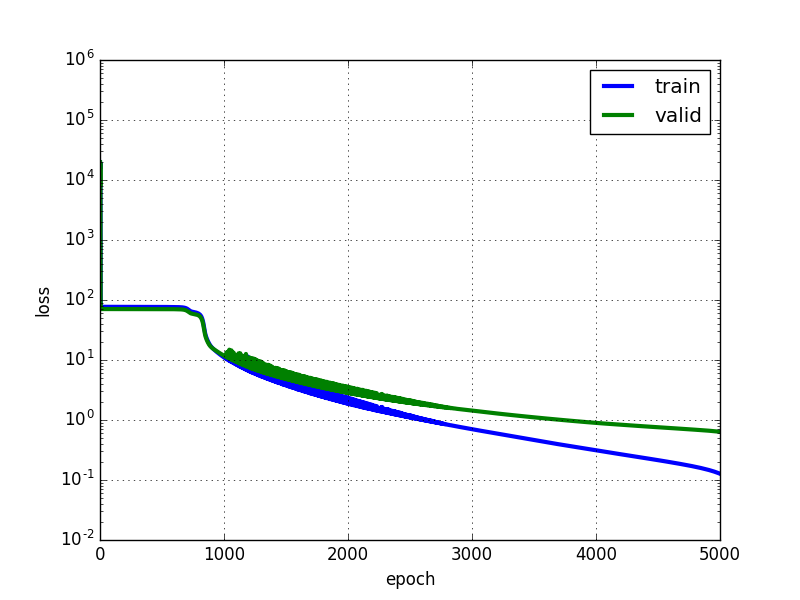
\includegraphics[width=0.4\textwidth]{./images/figure_1_cnn3_5000_loss_v11}}~~
\subfloat[rule\_2]{\label{}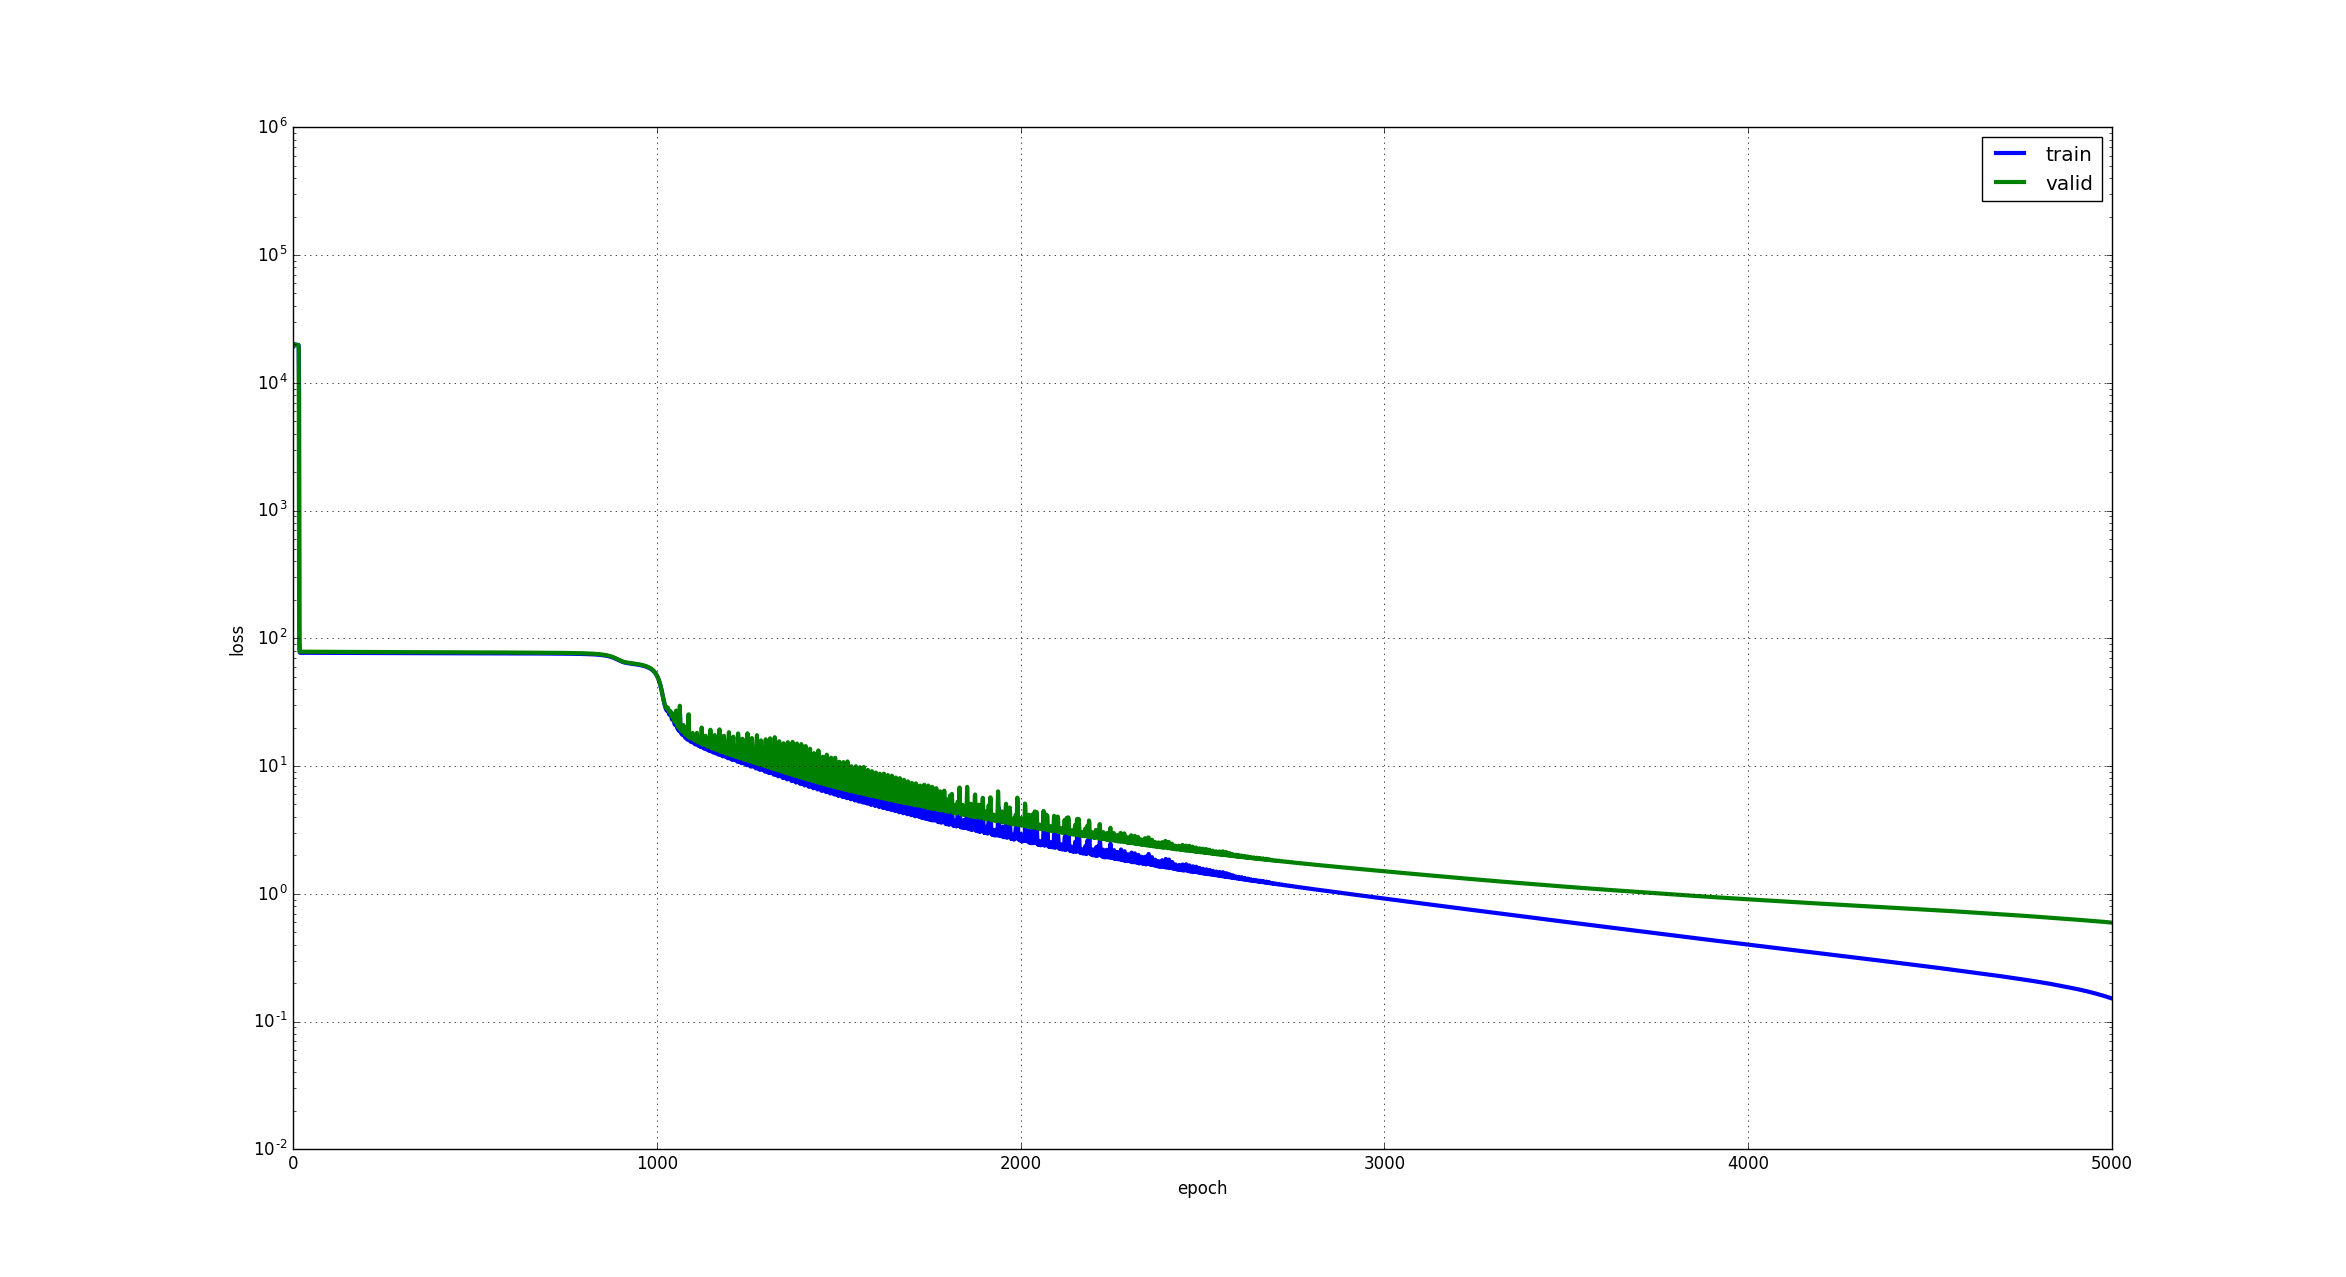
\includegraphics[width=0.4\textwidth]{./images/figure_1_cnn3_5000_loss_v12}}\\
\subfloat[rule\_3]{\label{}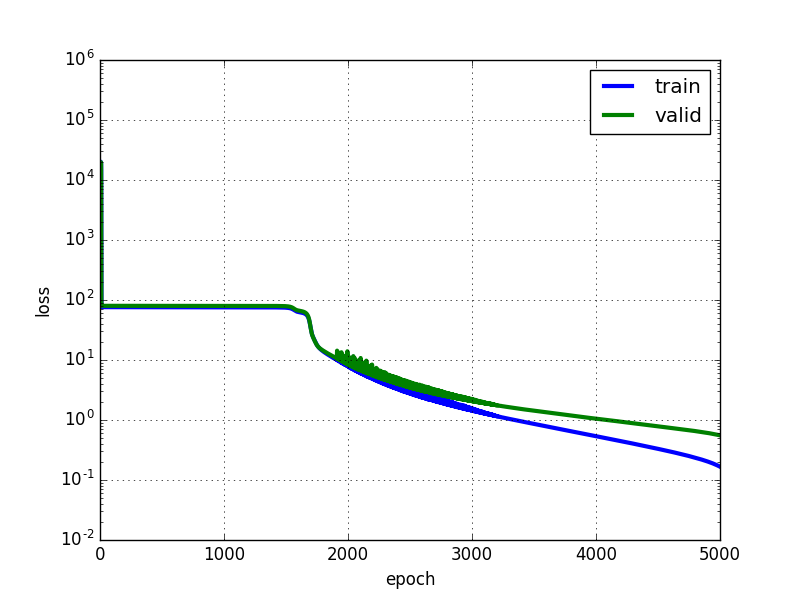
\includegraphics[width=0.4\textwidth]{./images/figure_1_cnn3_5000_loss_v13}}\\
\subfloat[rule\_4]{\label{}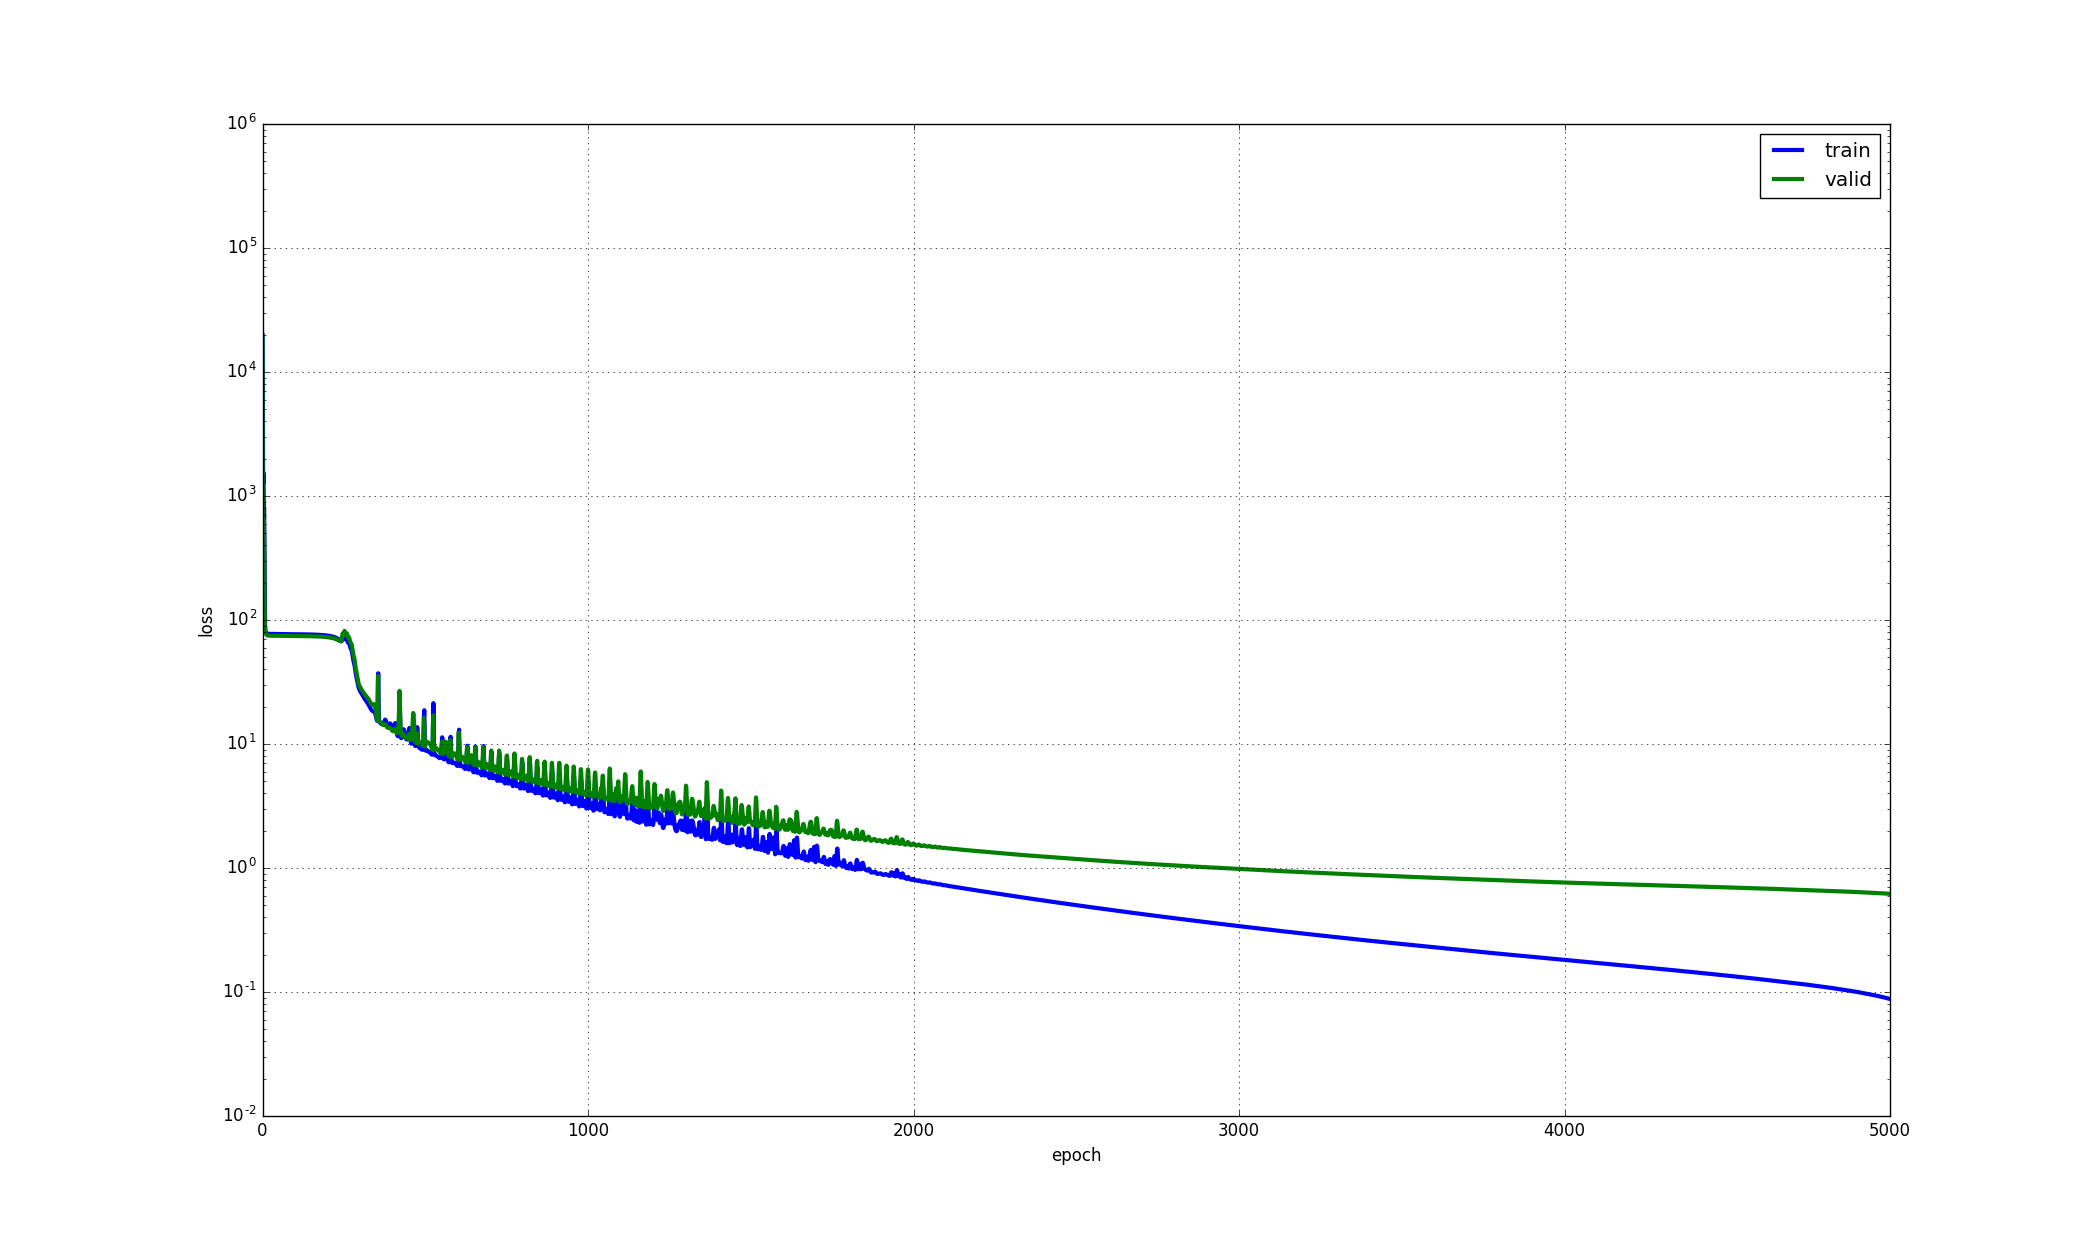
\includegraphics[width=0.4\textwidth]{./images/figure_1_cnn3_5000_loss_v14}}~~
\subfloat[rule\_5]{\label{}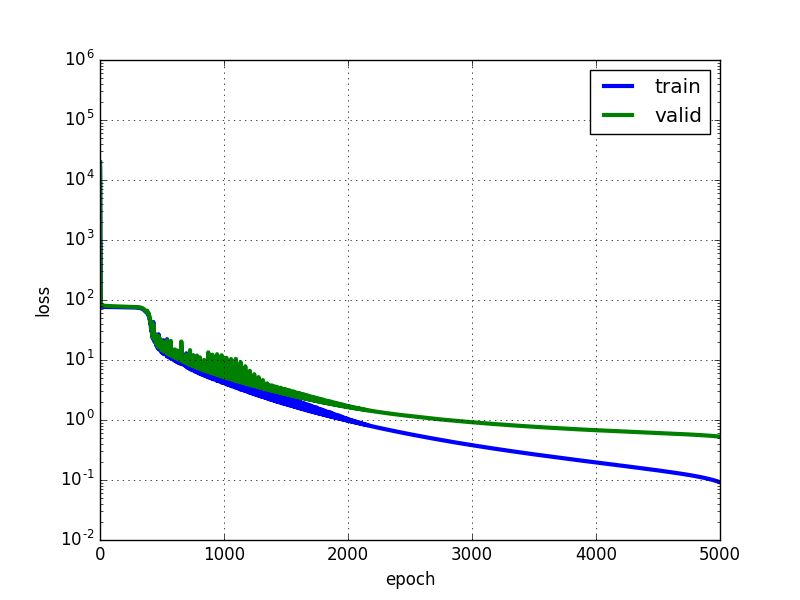
\includegraphics[width=0.4\textwidth]{./images/figure_1_cnn3_5000_loss_v15}}
\caption{The loss during training and validation followed each rule to choose data }
\label{cnn3l}
\end{figure}
\pagebreak

Fig.\ref{cnn3t} show the predicted positions on test dataset followed rule\_3:
%\begin{figure}[h!]
%	\centering
%	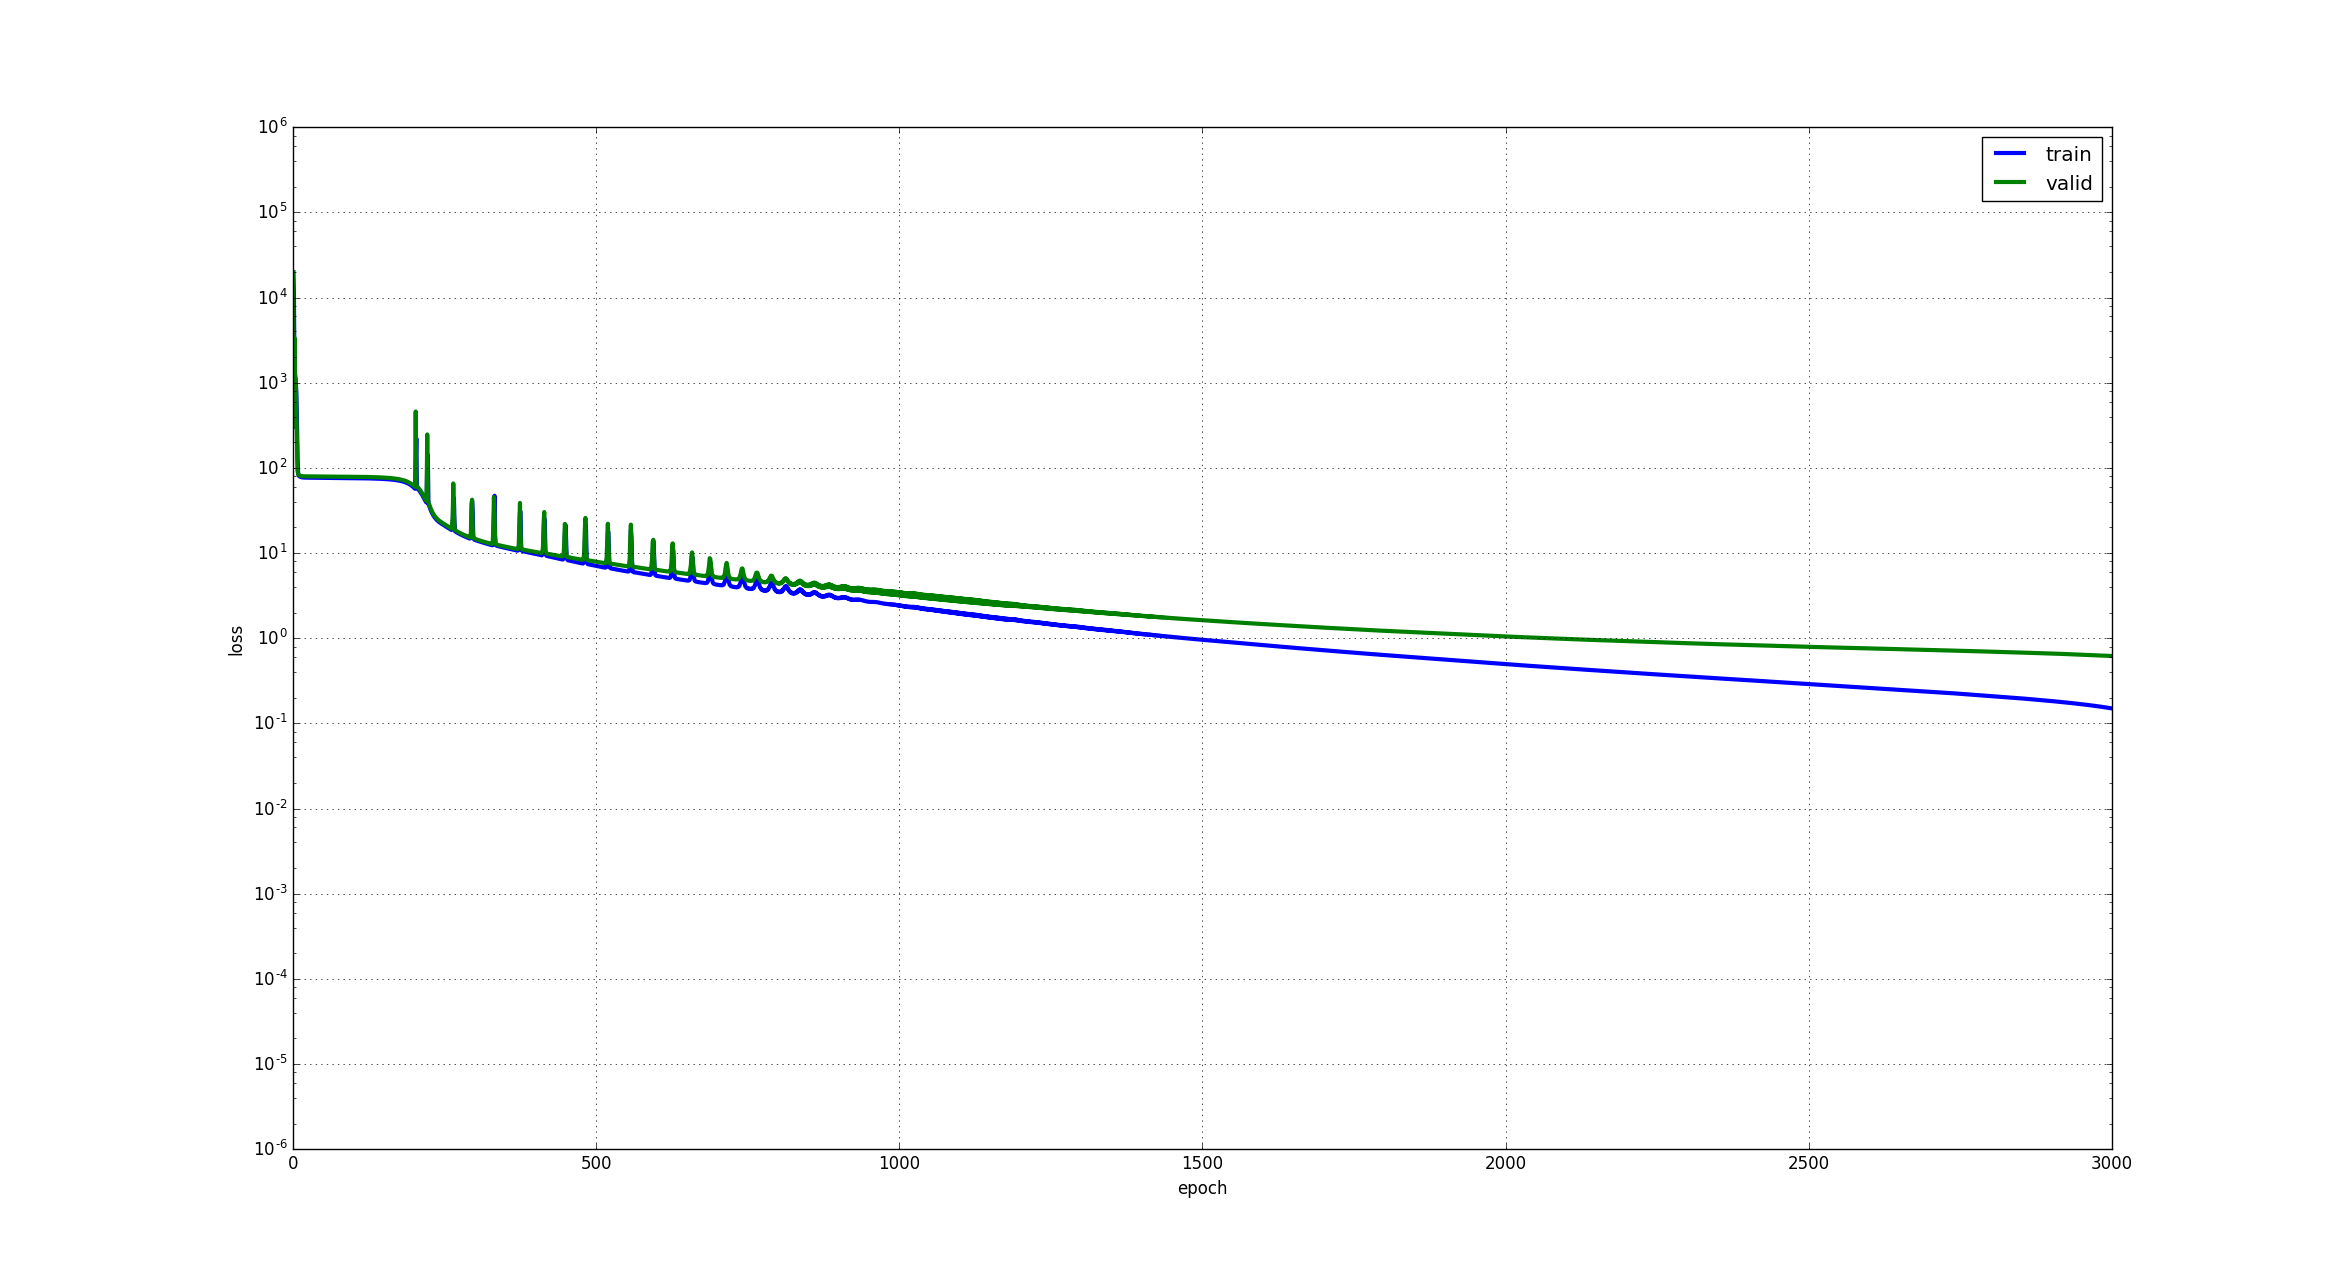
\includegraphics[scale=0.2]{images/figure_1_loss_cnn3_3000_2}
%	\caption{The loss during training and validation of rule\_1}
%	\label{cnn3l}
%\end{figure}
\begin{figure}[h!]
	\centering
	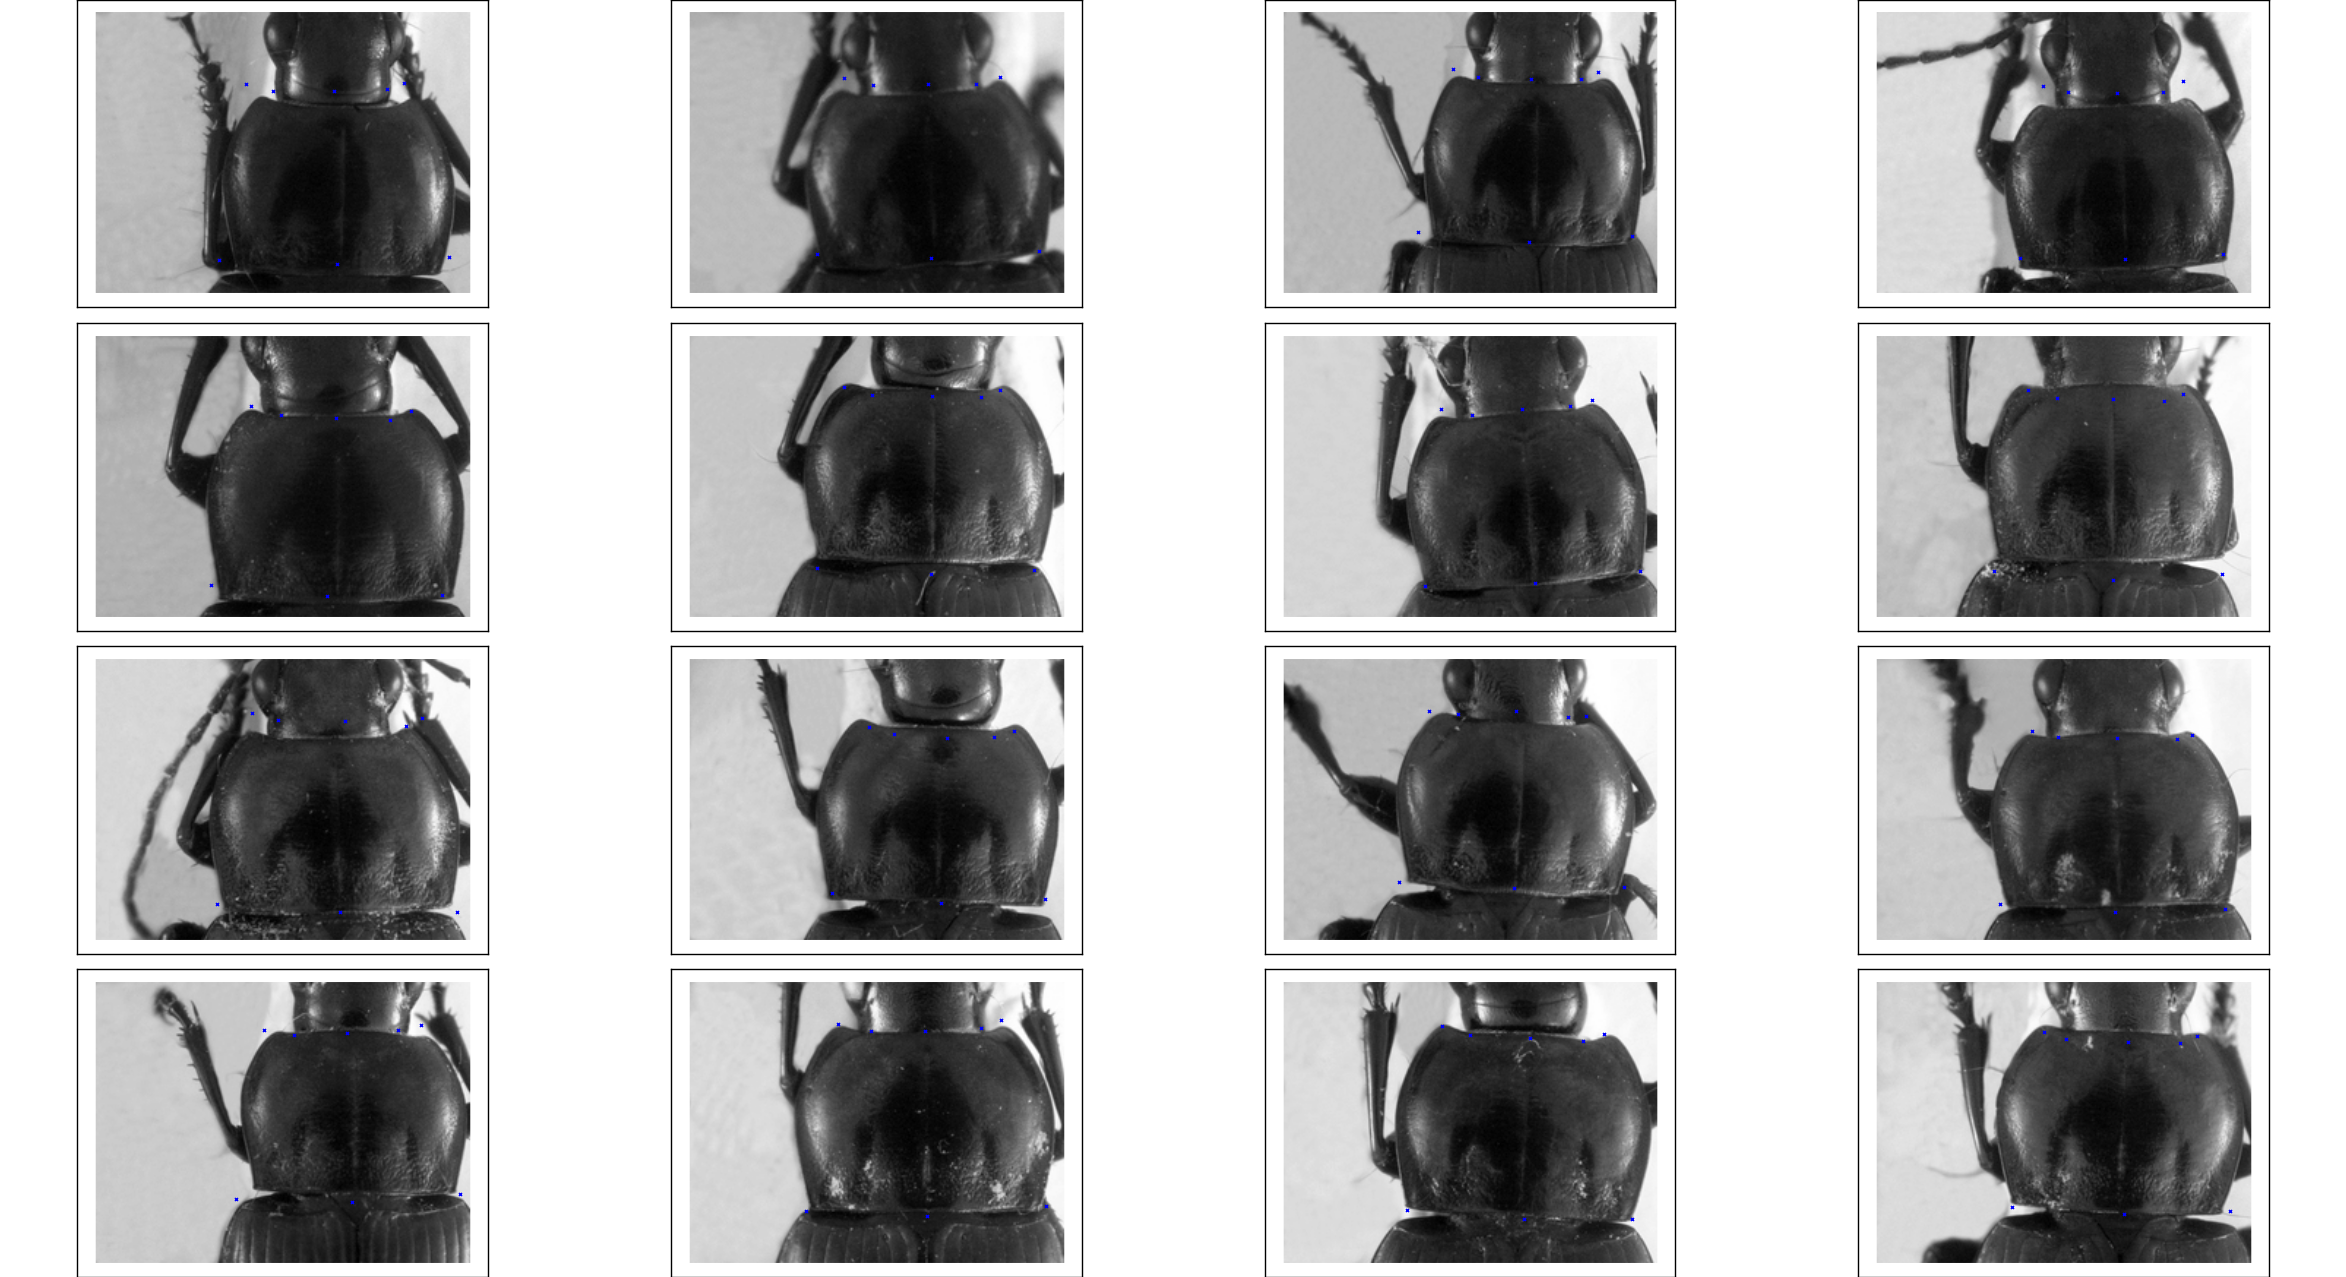
\includegraphics[scale=0.2]{images/figure_1_cnn3_5000_v13}
	\caption{The prediction landmarks on 16-pronotum images}
	\label{cnn3t}
\end{figure}~\\[2cm]
%\begin{figure}[h!]
%	\centering
%	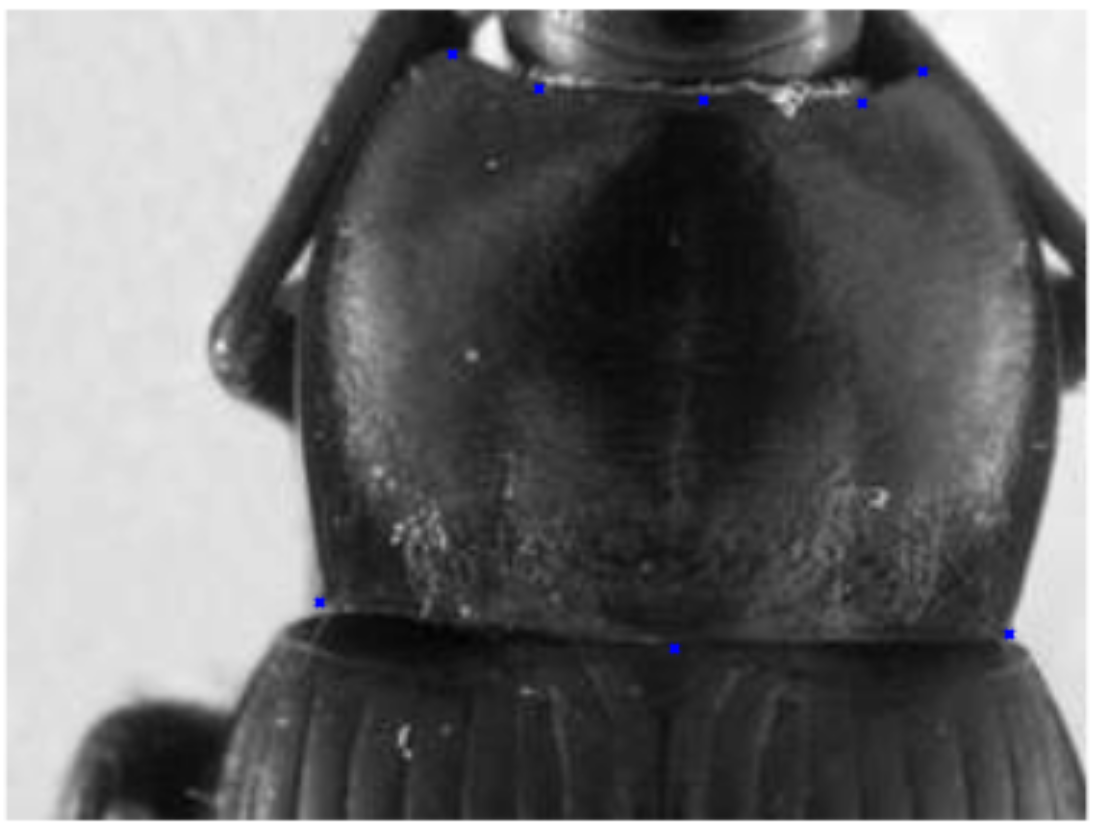
\includegraphics[scale=0.25]{images/plandmark}
%	\caption{The prediction landmarks on a pronotum}
%	\label{cnn3t1}
%\end{figure}
The network in model 3 is applied to predict the landmarks on tete and elytre with some modifications such as: the output at the last of full connected layer. The data that used to train and test are chosen by applying rule\_3. Table.\ref{tete},\ref{elytre} shown the statistic on the test set of tete and elytre by different correlation coefficient methods:
\begin{table}[h!]
	\centering
	\begin{tabular}{l c c}
		Method & x correlation & y correlation \\ \hline
		Pearson & $0.99082758$ & $0.988833$ \\ \hline
		Spearman & $0.9868292$ & $0.989447$ \\ \hline
		Kendall & $0.905933$ & $0.9130359$ \\ \hline
	\end{tabular}
	\caption{The correlation between manual and predicted landmarks on tete images}
	\label{tete}
\end{table}
\begin{table}[h!]
	\centering
	\begin{tabular}{l c c}
		Method & x correlation & y correlation \\ \hline
		Pearson & $0.984969$ & $0.9976646$ \\ \hline
		Spearman & $0.9840307$ & $0.966091$ \\ \hline
		Kendall & $0.8996806$ & $0.846849$ \\ \hline
	\end{tabular}
	\caption{The correlation between manual and predicted landmarks on elytre images}
	\label{elytre}
\end{table}~\\
From the result of Table \ref{losschoosedata}, the dataset which was chosen by rule\_3 is used to continue the experiments. To improve the results, we have modified the rule to pre-process the input data: the target (coordinates of manual landmarks) is normalized into the range of $[-1,1]$, instead of $[0,256]$ for x-coordinate and $[0,192]$ for y-coordinate. Additional, the \textit{learning rate} of the network has been changed to increase the speed of training process.

After changing, the result that we obtain as we expect: training loss and validation loss have decreased significantly(training loss: \textbf{0.00002}, validation loss: \textbf{0.00012}). Thus, the landmarks coordinates have been normalized into $[-1,1]$, so, to calculate the MSE error, we will take the square error and multiply by scale ratio again: the error is arround $1.4$(validation loss). Fig.\ref{tvlscaletarget} shows the losses during training and validation. We can see that overfitting have appeared during the train and validation processes.
\begin{figure}[h!]
	\centering
	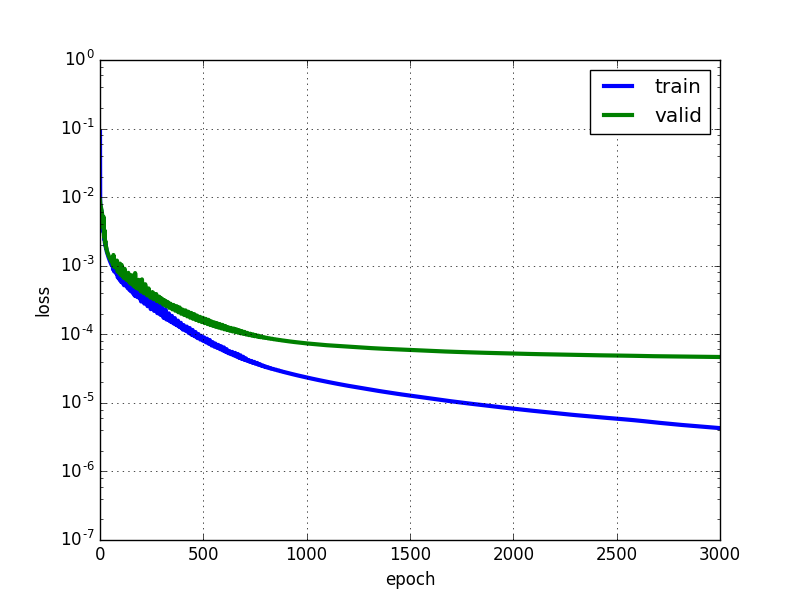
\includegraphics[scale=0.5]{images/figure_1_cnn3_3000_v13_loss_change2}
	\caption{The training and validation loss when normalize the landmarks coordinates}
	\label{tvlscaletarget}
\end{figure}~\\
To prevent the overfitting on the network, we have modified both data and model: on data side, we have changed the \textit{split} ratio to get more samples for validation set($40\%$ instead of $20\%$ of number of samples); on model side, the number of units in the last two hidden layers (full-connected layer) are increased from 500 to 1000. Besides, four dropout layers have been added into the network. They have been located following the pooling layers and the first full-connected layer. The dropout ratios are $0.1$, $0.2$, $0.3$ and $0.5$ (Fig.\ref{model3dropout}).
\begin{figure}[h!]
	\centering
	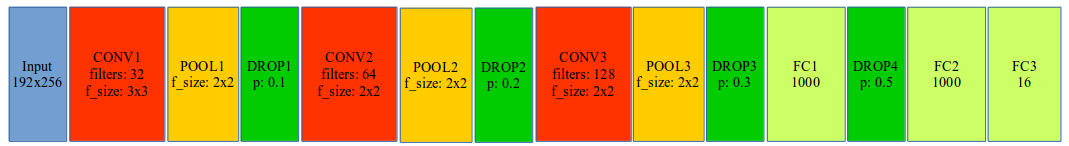
\includegraphics[scale=0.35]{images/model3_dropout}
	\caption{The proposed model with dropout layers}
	\label{model3dropout}
\end{figure}~\\
Fig.\ref{tvldropout} shows the losses after the model have been modified. The overfitting problem is solved but the losses are stability from $2000^{th}$ until the end(we need more data). Table.\ref{coffdropout} shows the correlation coefficient of new model. Clearly that, the result have been improved a little bit when we compare with the last result. 
\begin{figure}[h!]
	\centering
	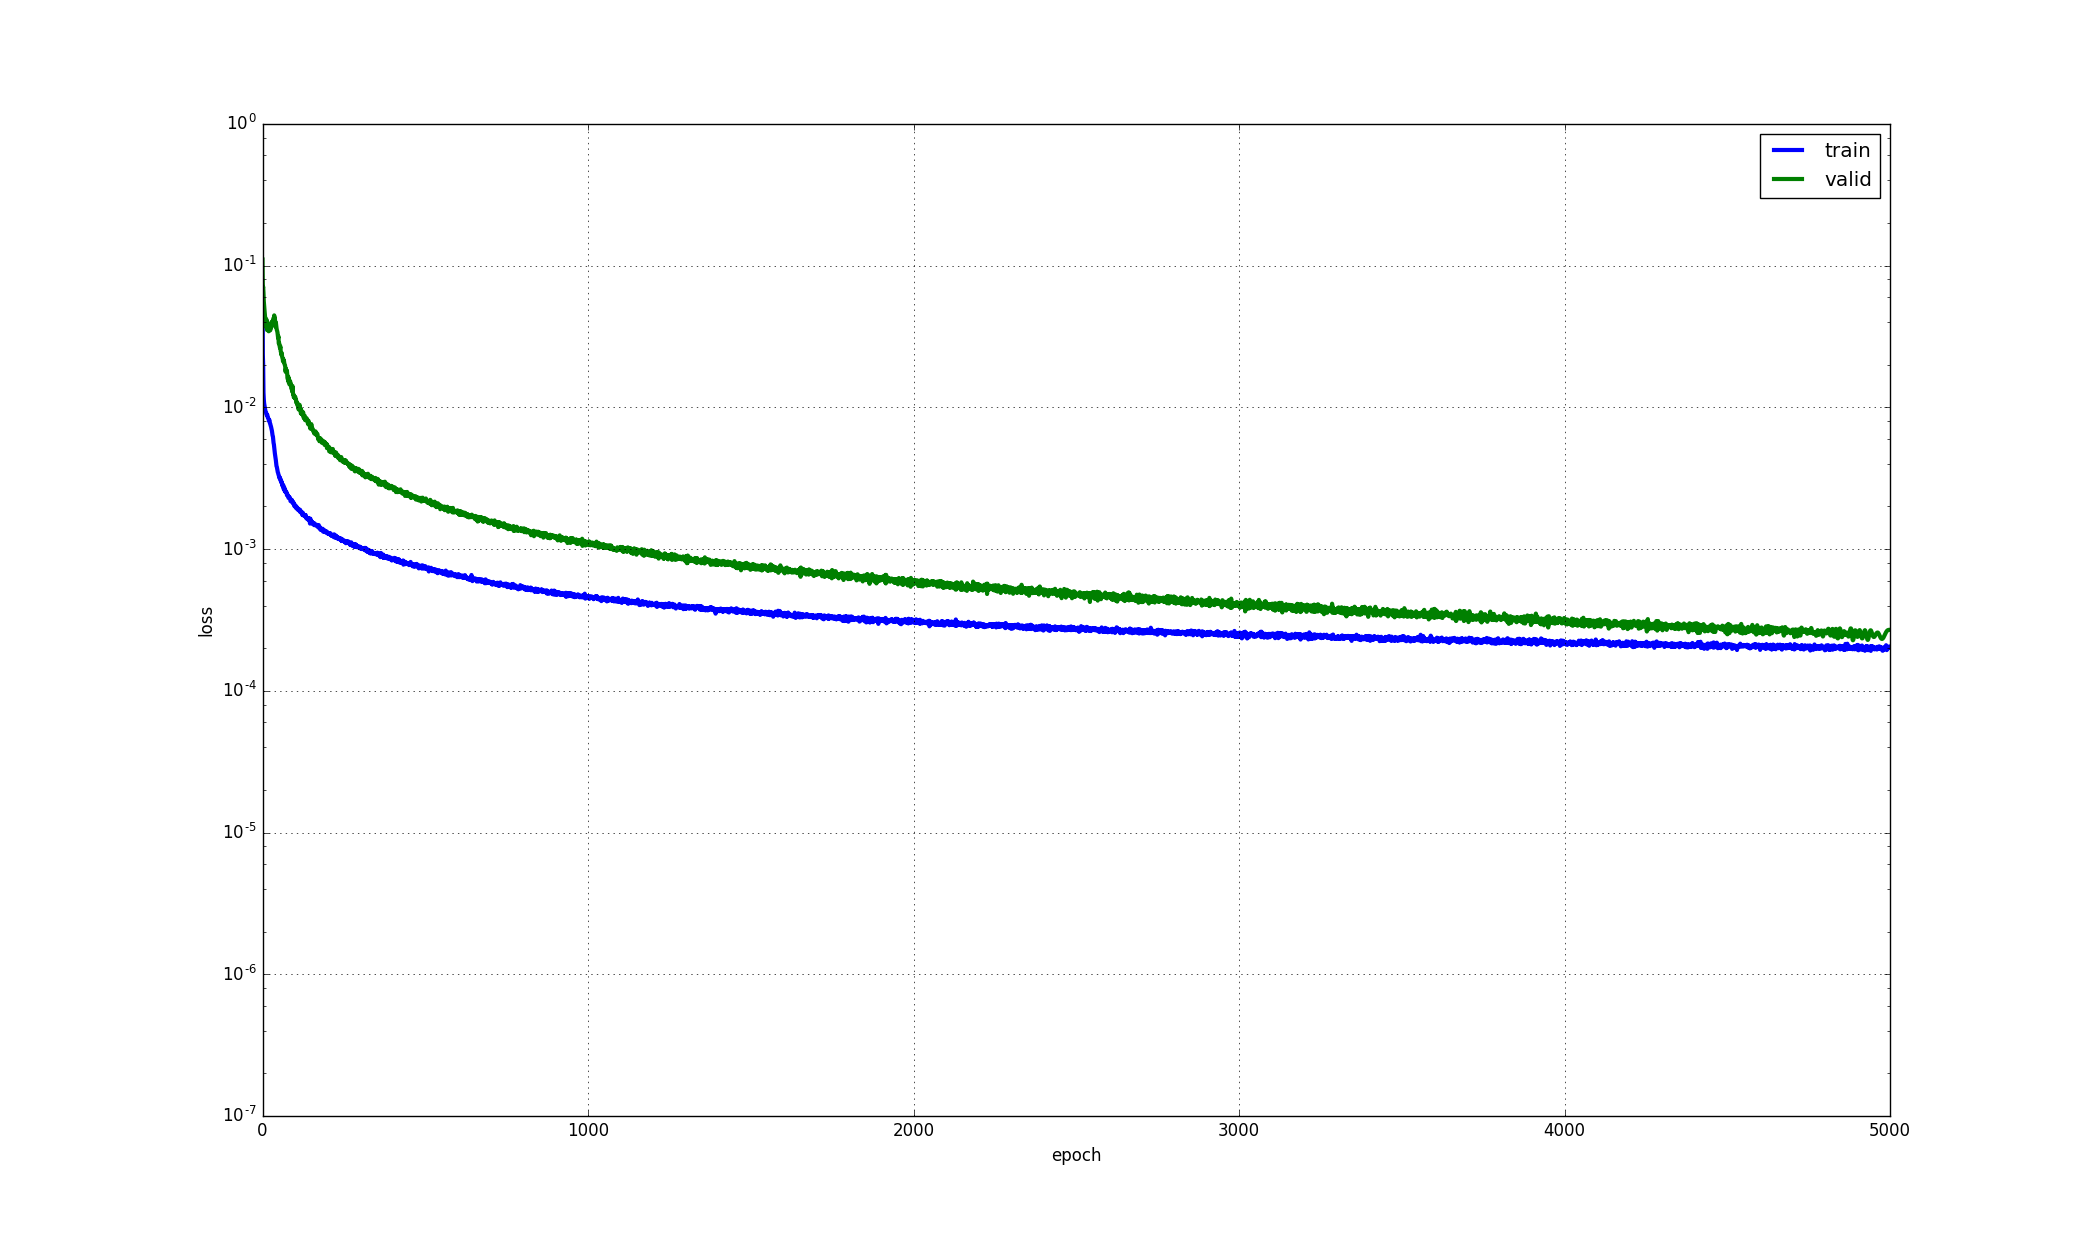
\includegraphics[scale=0.2]{images/figure_1_cnn3_3000_v13_loss_change3_dropout_increase_2}
	\caption{The training and validation loss with dropout layers}
	\label{tvldropout}
\end{figure}~\\
\begin{table}[h!]
	\centering
	\begin{tabular}{l c c}
		Method & x correlation & y correlation \\ \hline
		Pearson & $0.9970585$ & $0.9978605$ \\ \hline
		Spearman & $0.9942475$ & $0.9859642$ \\ \hline
		Kendall & $0.9430501$ & $0.9067739$ \\ \hline
	\end{tabular}
	\caption{The correlation between manual and predicted landmarks on pronotum images with new model}
	\label{coffdropout}
\end{table}
\section{Conclusions}
In this studied, two methods that used to predict the landmarks on 2D gray-scale images are studied. For each case, the model is suitable with different dataset but the results are still not good when we change the data (pronotum). Besides, we proposed a network to learn and detect the landmark positions on pronotum. The accuracy of the model is greater than $98 \%$. The results are evaluated on 3 datasets: pronotum, tete and elytre. From the correlation coefficients of each dataset shows that if we consider on the statistic side, the coefficients are enough good to precise. But when we see the real position on each image, that is not good as we expect. It means the model is not really suitable for the problem and we need to improve the model.
\bibliographystyle{unsrt}
\bibliography{includes/references}


\end{document}